
%<<setup-child, include = FALSE>>=
%library(knitr)
%set_parent("../style/preamble.Rnw")
%options(digits = 16)
%@
\input{../../2021/style/preamble4tex}
% dependencies: amsmath, amssymb, dsfont
% math spaces
\ifdefined\N
\renewcommand{\N}{\mathds{N}} % N, naturals
\else \newcommand{\N}{\mathds{N}} \fi
\newcommand{\Z}{\mathds{Z}} % Z, integers
\newcommand{\Q}{\mathds{Q}} % Q, rationals
\newcommand{\R}{\mathds{R}} % R, reals
\ifdefined\C
\renewcommand{\C}{\mathds{C}} % C, complex
\else \newcommand{\C}{\mathds{C}} \fi
\newcommand{\continuous}{\mathcal{C}} % C, space of continuous functions
\newcommand{\M}{\mathcal{M}} % machine numbers
\newcommand{\epsm}{\epsilon_m} % maximum error

% counting / finite sets
\newcommand{\setzo}{\{0, 1\}} % set 0, 1
\newcommand{\setmp}{\{-1, +1\}} % set -1, 1
\newcommand{\unitint}{[0, 1]} % unit interval

% basic math stuff
\newcommand{\xt}{\tilde x} % x tilde
\newcommand{\argmin}{\mathop{\mathrm{arg\,min}}} % argmin
\newcommand{\argmax}{\mathop{\mathrm{arg\,max}}} % argmax
\newcommand{\argminlim}{\argmin\limits} % argmin with limits
\newcommand{\argmaxlim}{\argmax\limits} % argmax with limits
\newcommand{\sign}{\operatorname{sign}} % sign, signum
\newcommand{\I}{\mathbb{I}} % I, indicator
\newcommand{\order}{\mathcal{O}} % O, order
\newcommand{\bigO}{\mathcal{O}} % Big-O Landau
\newcommand{\littleo}{{o}} % Little-o Landau
\newcommand{\pd}[2]{\frac{\partial{#1}}{\partial #2}} % partial derivative
\newcommand{\floorlr}[1]{\left\lfloor #1 \right\rfloor} % floor
\newcommand{\ceillr}[1]{\left\lceil #1 \right\rceil} % ceiling
\newcommand{\indep}{\perp \!\!\! \perp} % independence symbol

% sums and products
\newcommand{\sumin}{\sum\limits_{i=1}^n} % summation from i=1 to n
\newcommand{\sumim}{\sum\limits_{i=1}^m} % summation from i=1 to m
\newcommand{\sumjn}{\sum\limits_{j=1}^n} % summation from j=1 to p
\newcommand{\sumjp}{\sum\limits_{j=1}^p} % summation from j=1 to p
\newcommand{\sumik}{\sum\limits_{i=1}^k} % summation from i=1 to k
\newcommand{\sumkg}{\sum\limits_{k=1}^g} % summation from k=1 to g
\newcommand{\sumjg}{\sum\limits_{j=1}^g} % summation from j=1 to g
\newcommand{\summM}{\sum\limits_{m=1}^M} % summation from m=1 to M
\newcommand{\meanin}{\frac{1}{n} \sum\limits_{i=1}^n} % mean from i=1 to n
\newcommand{\meanim}{\frac{1}{m} \sum\limits_{i=1}^m} % mean from i=1 to n
\newcommand{\meankg}{\frac{1}{g} \sum\limits_{k=1}^g} % mean from k=1 to g
\newcommand{\meanmM}{\frac{1}{M} \sum\limits_{m=1}^M} % mean from m=1 to M
\newcommand{\prodin}{\prod\limits_{i=1}^n} % product from i=1 to n
\newcommand{\prodkg}{\prod\limits_{k=1}^g} % product from k=1 to g
\newcommand{\prodjp}{\prod\limits_{j=1}^p} % product from j=1 to p

% linear algebra
\newcommand{\one}{\bm{1}} % 1, unitvector
\newcommand{\zero}{\mathbf{0}} % 0-vector
\newcommand{\id}{\bm{I}} % I, identity
\newcommand{\diag}{\operatorname{diag}} % diag, diagonal
\newcommand{\trace}{\operatorname{tr}} % tr, trace
\newcommand{\spn}{\operatorname{span}} % span
\newcommand{\scp}[2]{\left\langle #1, #2 \right\rangle} % <.,.>, scalarproduct
\newcommand{\mat}[1]{\begin{pmatrix} #1 \end{pmatrix}} % short pmatrix command
\newcommand{\Amat}{\mathbf{A}} % matrix A
\newcommand{\Deltab}{\mathbf{\Delta}} % error term for vectors

% basic probability + stats
\renewcommand{\P}{\mathds{P}} % P, probability
\newcommand{\E}{\mathds{E}} % E, expectation
\newcommand{\var}{\mathsf{Var}} % Var, variance
\newcommand{\cov}{\mathsf{Cov}} % Cov, covariance
\newcommand{\corr}{\mathsf{Corr}} % Corr, correlation
\newcommand{\normal}{\mathcal{N}} % N of the normal distribution
\newcommand{\iid}{\overset{i.i.d}{\sim}} % dist with i.i.d superscript
\newcommand{\distas}[1]{\overset{#1}{\sim}} % ... is distributed as ...


\begin{document}

\lecturechapter{3}{Numerical Error \& Conditioning}
\lecture{CIM1 Statistical Computing}




%\section{Error \& Condition}

\begin{vbframe}{Numerical Error}

\begin{center}
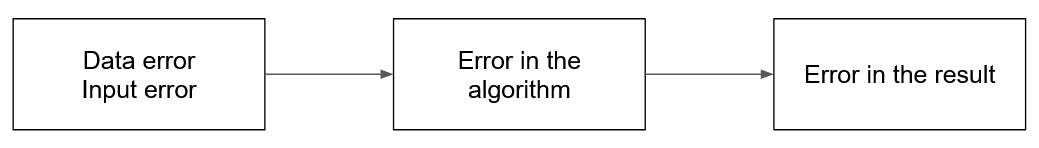
\includegraphics{figure_man/error_sources.PNG}
\end{center}

Errors in the result are caused by
\begin{itemize}
\item Data error or input error; often unavoidable, are part of the problem \\ $\to$ \textbf{Condition of the problem}
\item Error in the algorithm that can often be fixed by modification \\ $\to$ \textbf{Stability of algorithms}
\end{itemize}


\framebreak

Given: Approximate value $\tilde x$ for exact value $x$.

\begin{itemize}
\item Absolute error (this is signed!):
$$
  \Delta x = \tilde x - x
$$

If $|\Delta x| \le \epsilon$, then $\epsilon$ is known as absolute error bound.

\item Relative error:
$$
  \delta_x = \frac{|\tilde x - x|}{|x|} = \frac{|\Delta x|}{|x|}\qquad
  % \mbox{und} \qquad \tilde \delta = \frac{\tilde x - x}{\tilde x}
$$
If $\delta_x \le \rho$, then $\rho$ is known as relative error bound.
\end{itemize}

\textbf{Comment:}

Relative error is dimensionless, value in denominator
may obviously not be too close to zero ($\to$ use absolute error instead).


\framebreak

The following holds:
\begin{eqnarray*}
  \label{eq:1}
  \tilde x &=& x \left(1+\frac{\Delta x}{x}\right)
  % \tilde x &=& x (1-\tilde\delta)^{-1}
\end{eqnarray*}
% und wegen
% $$
  % (1-\tilde\delta)^{-1} = 1 + \tilde\delta + \tilde\delta^2 + \ldots
  % \approx 1+\tilde\delta
% $$
% ist die Verwendung von $\delta$ und $\tilde\delta$ in erster
% Ndherung dquivalent.

If only the first $m$ digits of a number are determined in decimal representation,
a possible relative error of $10^{-m}$ results (and vice versa).

\framebreak

% \begin{itemize}
%  \item Beim gemeinsamen Auftreten mehrerer \emph{gleichartiger}
%   Grv_en, kann eine \emph{gemeinsame Vergleichsgrv_e} sinnvoll sein
%   (Mittelwert, Maximum, \ldots).
%  \item für Vektor $\xv = (x_1, \ldots, x_n)^\top$ gleichartiger Grv_en Norm als
%    Vergleichsgrv_e:
%    $$
%    \frac{1}{\|\xv\|} (\tilde{\xv} - \xv) \qquad \text{bzw.} \qquad
%      \frac{1}{\|\xv\|}(\|\tilde{\xv} - \xv\|)
%    $$
%  \item für Vektor $\xv = (x_1, \ldots, x_n)^\top$ verschiedenartiger Grv_en:
%    $$
%    \delta_{\xv} = \left( \frac{\tilde{x}_1 - x_1}{x_1}, \ldots, \frac{\tilde{x}_n - x_n}{x_n} \right)^\top
%     \qquad \text{bzw.} \qquad \|\delta_{\xv}\|
%    $$
% \end{itemize}

% \framebreak

% \textbf{Beispiel:} $x + y$,

% \lz

% mit $\tilde{x} = f(x) = x(1 + \delta_x)$ und $\tilde{y} = f(y) = y(1 + \delta_y)$.

% \lz

% Ergebnis:

% \lz

% $f(f(x) + f(y)) = (f(x) + f(y))(1 + \delta_e)$ und $\max\{|\delta_x|, |\delta_y|, |\delta_e|\} \leq \epsm$.
% \begin{eqnarray*}
% |f(f(x) + f(y)) - (x + y)| &=& |(f(x) + f(y))(1 + \delta_e) - x - y| \\
% &=& |f(x) + f(y) + f(x)\delta_e + f(y)\delta_e - x - y| \\
% &=& |f(x) - x + f(y) - y + \delta_e(f(x) + f(y))| \\
% &=& |\delta_x x + \delta_y y + \delta_e(x(1 + \delta_x) + y(1 + \delta_y))| \\
% &\leq& |\epsm x + \epsm y + \epsm((x + y)(1 + \epsm))| \\
% &=& |\epsm(x + y) + (x + y)(\epsm + \epsm^2)| \\
% &\approx& 2 \epsm|x + y|
% \end{eqnarray*}
\end{vbframe}


\begin{vbframe}{Condition of a problem}

\begin{center}
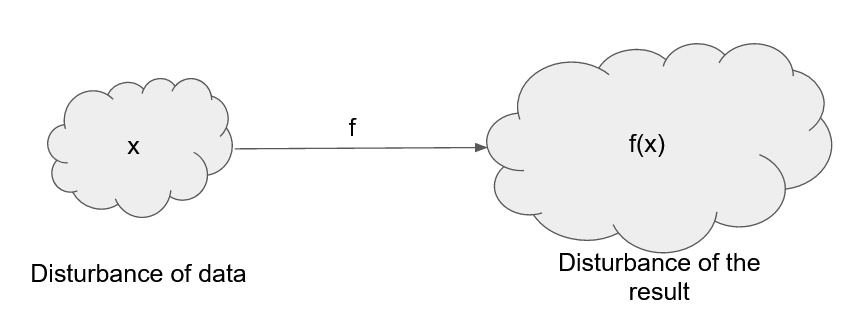
\includegraphics[width = .6\textwidth]{figure_man/condition_eng.PNG}
\end{center}

How sensitive is the result to a small disturbance of the data?

\begin{description}
 \item[Well-conditioned:] Result is a little sensitive
 \item[Ill-conditioned:] Result is very sensitive
\end{description}

This is particularly important in statistics, since data is usually error-prone.

% \lz
%
% In Anwendungen werden hdufig gut konditionierte Verfahren als
% \emph{stabil} bezeichnet, schlecht konditionierte als
% \emph{instabil}.
%
% \lz
%
% Unterschied, ob das Problem schlecht konditioniert ist (dann ist jedes
% Verfahren instabil), oder ob das Verfahren instabil ist, obwohl das Problem gut
% konditioniert ist.

\framebreak

\textbf{Example 1: }System of equations

\begin{eqnarray*}
0.835x + 0.667y &=& 0.168 \\
0.333x + 0.266y &=& 0.067
\end{eqnarray*}
The solution is $x = 1$ and $y = -1$.

\lz

By a small change of the right side, for example $0.067~\to~0.066$, the solution changes to
$x = -666$ and $y = 834$.

\framebreak

\textbf{Example 2: }Intersection of two straight lines

\begin{center}

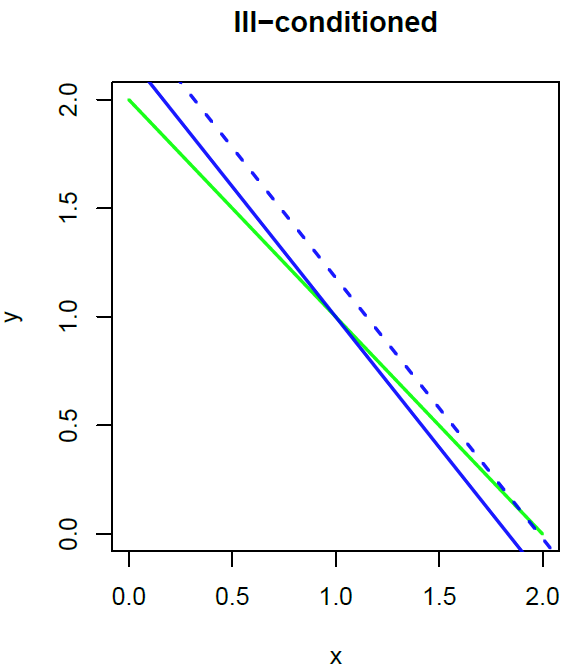
\includegraphics[width = 0.4\linewidth]{figure_man/ill-con.png} ~~~ 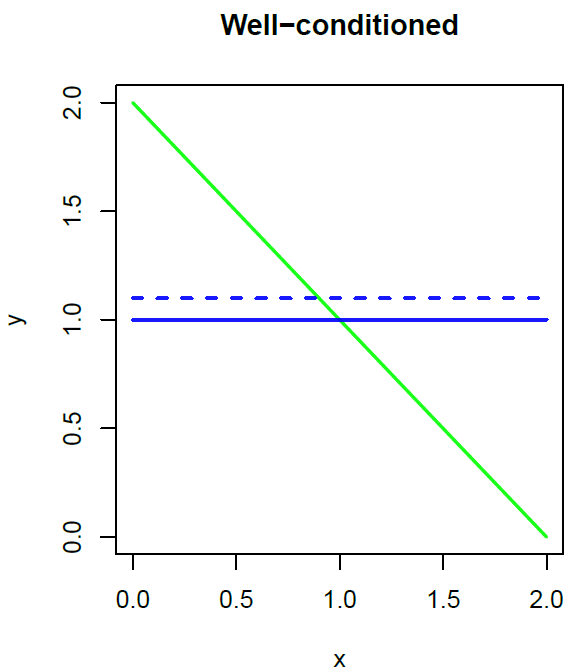
\includegraphics[width = 0.4\linewidth]{figure_man/well-con.png}

\end{center}

\vspace{0.2cm}

\begin{footnotesize}
In the left case (ill-conditioned problem) a small disturbance has a big influence on the solution (position of the intersection).
In the right case (well-conditioned) the disturbance has only a minor effect on the solution.
\end{footnotesize}

\end{vbframe}

\begin{vbframe}{Condition (Definition)}

Consider a problem of form $y = f(x)$. Condition describes to what extent the solution changes with minor data disturbance ($\tilde x = x + \delta x$).

\lz

\textbf{Condition number (at position x)}: the smallest $\kappa \geq 0$, so that

$$
\frac{|f(x+\Delta x)-y|}{|y|} \leq \kappa \ \frac{|\Delta x|}{|x|} \text{ for } \Delta x \to 0.
$$

The condition therefore compares the relative error of input and output.

A problem is

\begin{itemize}
\item Well-conditioned if $\kappa \not \gg 1$
\item Ill-conditioned if $\kappa \gg 1$
\item Ill-posed when $\kappa = \infty$
\end{itemize}

\begin{footnotesize}
Note that for machine numbers $\Delta x < \epsm$ (approximation error when importing data)!
\end{footnotesize}


%\begin{itemize}
%  \item Vergleich der relativen Fehler von Input und Output.
% \item  $\kappa$ gro_ $\SpAr$ \textbf{schlecht konditioniertes Problem}
% (schwierig)
%\end{itemize}
\end{vbframe}


\begin{vbframe}{Condition for vectors}

For vectors, errors are defined by means of a suitable norm.

\lz

\textbf{Absolute error:}
$$
  \Delta \xv = \tilde \xv - \xv
$$

\textbf{Relative error:}
$$
  \delta = \frac{\|\tilde \xv - \xv \|}{\|\xv\|} \qquad
  % \mbox{und} \qquad \tilde \delta = \frac{\tilde x - x}{\tilde x}
$$

Similarly, for $f:\R^n \rightarrow \R^d$ the \textbf{norm-wise} condition at the location $\xv$ is defined by using the condition number.

\lz

% Sei $\xv = (x_1,\dots,x_n)$, $\tilde{\xv} = (x_1+\delta_1,\dots,x_n+\delta_n)$ und
% $\yv = (y_1,\dots,y_d)$.
%
% \lz

\textbf{Condition number}: The smallest $\kappa \geq 0$, such that

$$
\frac{\|f(\xv+\Delta \xv)-\yv\|}{\|\yv\|} \leq \kappa \ \frac{\|\Delta \xv\|}{\|\xv\|} \text{ for } \|\Delta \xv\| \to 0.
$$

Let $f: \R^n \to \R$ be differentiable in point $x$, the condition can be specified using the derivative:

\vspace*{-.3cm}
$$
\kappa =  \frac{\|\xv\|}{\|f(\xv)\|} \|\nabla f(\xv)\|.
$$

\lz
\vspace*{0.5cm}
\begin{footnotesize}
\textbf{Proof sketch:}

The definition of the condition can be written as

\vspace*{-.3cm}
\begin{eqnarray*}
\kappa &=& \limsup_{\|\Delta \xv\| \to 0} \frac{\|f(\xv + \Delta \xv)-\yv\|}{\|\yv\|} \frac{\|\xv\|}{\|\Delta \xv\|}  = \limsup_{\|\Delta \xv\|\to 0} \frac{\|f(\xv + \Delta \xv)-\yv\|}{\|\Delta \xv\|} \frac{\|\xv\|}{\|f(\xv)\|} 
\end{eqnarray*}

According to the mean value theorem the following applies: there is a $\bm{v} \in (\bm{0}, \Delta \xv)$ such that

$$
\nabla f(\xv + \bm{v}) = \frac{\|f(\xv + \Delta \xv)-\yv\|}{\|\Delta \xv\|}.
$$
\vspace*{0.5cm}
From $\|\Delta \xv\| \to 0$ follows $\|\bm{v}\|\to 0$ and thus
\begin{eqnarray*}
\kappa &=& \limsup_{\|\Delta \xv\| \to 0} \|\nabla f(\xv + \bm{v})\| \frac{\|\xv\|}{\|f(\xv)\|} = \|\nabla f(\xv)\| \frac{\|\xv\|}{\|f(\xv)\|}
\end{eqnarray*}
\end{footnotesize}


\begin{itemize}
\item $\nabla f(\xv)$ corresponds to the $1 \times n$ Jacobi matrix here. Thus, $\|\nabla f(\xv)\|$ is an induced \emph{matrix norm}.
\item The condition depends on the choice of the vector norm / induced matrix norm.
\end{itemize}


\end{vbframe}

% \begin{vbframe}{Komponentenweise Kondition}
%
% \normalsize
% Eine alternative Definition zur  Kondition ist die \textbf{komponentenweise} Kondition.
%
% \lz
%
% \textbf{Konditionszahl}: Das kleinste $\kappa_{rel} \geq 0$, so dass
%
% $$
% \frac{\|f(\xv + \Delta \xv)-\yv\|_\infty}{\|\yv\|_\infty} \leq \kappa_{rel} \ \max_i \frac{|\Delta x_i|}{|x_i|} \text{ für } \|\Delta \xv\| \to 0.
% $$
% % \begin{itemize}
% %  \item  $\kappa$ gro_ $\SpAr$ \textbf{schlecht konditioniertes Problem} (schwierig)
% % \end{itemize}
%
%
% \end{vbframe}
\begin{vbframe}{Arithmetic operations}

\begin{itemize}

 \item \textbf{Multiplication:}

We look at $f(x_1, x_2) = x_1 \cdot x_2$ and calculate $\kappa$ using

$$
\kappa = \frac{\|\nabla f(\xv)\|_1 \cdot \|\xv\|_1}{|f(\xv)|}
$$

Since

\vspace*{-.5cm}

\begin{eqnarray*}
\|\nabla f(\xv)\|_1 &=& \|(x_2, x_1)\|_1 \overset{*}{=} \max (|x_1|, |x_2|)\\\\
\|\xv\|_1 &=& \|(x_1, x_2)\|_1 = |x_1| + |x_2| \\\\
|f(\xv)| &=& |x_1 x_2|\\\
\end{eqnarray*}

\vspace*{-.5cm}

we get $\kappa = 1 + \frac{\max(|x_1|, |x_2|)}{\min(|x_1|, |x_2|)}$. So $\kappa$ becomes very big for $x_2 \ll x_1$.


\begin{footnotesize}
$^*$ Attention: induced matrix norm (maximum absolute column sum norm).
\end{footnotesize}

 \framebreak

% Eine \textbf{komponentenweise} Konditionsanalyse zeigt hingegen, dass die Multiplikation stets gut konditioniert ist:
%
%  \begin{eqnarray*}
% \frac{ |f(\xv + \Delta \xv) - y|}{|y|} &=& \frac{|(x_1 + \Delta x_1) (x_2 + \Delta x_2) - x_1x_2|}{|x_1x_2|} \\
%   &=& \frac{|x_1x_2 + x_1\Delta x_2 + x_2\Delta x_1 + \Delta x_1\Delta x_2 - x_1x_2|}{|x_1x_2|} \\
%   &\le& \frac{|\Delta x_1|}{|x_1|} + \frac{|\Delta x_2|}{|x_2|} + \frac{|\Delta x_1 \Delta x_2|}{|x_1 x_2|} \\
%   &\le&  2 \max_i \frac{|\Delta x_i|}{|x_i|}
%  \end{eqnarray*}
%
% für $\|\Delta \xv\| \to 0$.
%
% \framebreak


%  \item \textbf{Addition:}
%
%  \lz
%
%  $\quad y = x_1 + x_2,\quad \tilde y = (x_1 + \Delta x_1) + (x_2 + \delta_2)$
%  \begin{eqnarray*}
%  \SpAr \frac{\tilde y - y}{y} &=& \frac{\delta_1 + \delta_2}{x_1 + x_2} \\
%    &=& \frac{x_1}{x_1 + x_2}\ \frac{\delta_1}{x_1} +  \frac{x_2}{x_1 + x_2}\ \frac{\delta_2}{x_2}
%  \end{eqnarray*}
%  Schlecht konditioniert, falls $x_1 + x_2$ nahe bei 0 ($\kappa$ wird beliebig groß).
%
%  \lz
%
% Entspricht gerade dem Problem der \textbf{Auslöschung}.

\item \textbf{Addition / Subtraction: }

We will consider $f(x_1, x_2) = x_1 \pm x_2$ and calculate $\kappa$ using

$$
\kappa = \frac{\|\nabla f(\xv)\|_1 \cdot \|\xv\|_1}{|f(\xv)|}
$$

Since

\vspace*{-.5cm}

\begin{eqnarray*}
\|\nabla f(\xv)\|_1 &=& \|(1, \pm 1) \|\overset{*}{=} 1 \\\
\|\xv\|_1 &=& \|(x_1, x_2)\|_1 = |x_1| + |x_2| \\\
|f(\xv)| &=& |x_1 \pm x_2|\\\
\end{eqnarray*}

\vspace*{-.5cm}

we get $\kappa = \frac{|x_1| + |x_2|}{|x_1 \pm x_2|}$.

\lz

\begin{footnotesize}
$^*$ Attention: induced matrix norm (maximum absolute column sum norm).
\end{footnotesize}

\framebreak

The addition of two positive numbers is well-conditioned with $\kappa = \frac{|x_1| + |x_2|}{|x_1 + x_2|} = 1$.

\lz

In the case of $x_1 \approx x_2$, the subtraction of two positive numbers is very ill-conditioned  ($\kappa = \frac{|x_1| + |x_2|}{|x_1 + (- x_2)|}$ becomes arbitrarily large).
\lz

This problem is known as \textbf{loss of significance}.

\end{itemize}

\end{vbframe}


\begin{vbframe}{Loss of significance (example)}

\footnotesize
\begin{verbbox}
x = 1.234567890123456
y = 1.234567890000000
\end{verbbox}
\col

\normalsize
\lz
Theoretically we should get a result of \texttt{1.23456e-10} for the difference $x - y$. But the computer returns
\lz
\footnotesize
\begin{verbbox}
x - y

## [1] 1.234561342045026e-10
\end{verbbox}
\col
\lz
\lz
\normalsize
Why is this the case?

\framebreak

The numbers $x, y$ cannot be represented exactly in floating point notation, but only as a rounded number with $16$ significant digits. This inaccurate representation results in \enquote{uncertainties} from the 17th decimal place on.

\lz
\lz
\footnotesize
\begin{verbbox}
sprintf("%.20f", x)
## [1] "1.23456789012345602430"
\end{verbbox}
\col

\vspace{0.1cm}
\begin{verbbox}
sprintf("%.20f", y)
## [1] "1.23456788999999989009"
\end{verbbox}
\col
\lz
\framebreak
\normalsize
By subtracting the two numbers, the first $10$ significant digits cancel each other out. The uncertainties from the 17th place now shift to the 7th significant place.

\lz

Due to the loss of significance we have lost $10 = 16 - 6$ digits (number of significant digits - number of deleted digits) in accuracy.
\vspace*{-0.5cm}

\begin{align*}
   1.234567890123456???... & \\
 - 1.234567890000000???... & \\[-1ex]
 \rule{4.5cm}{0.4pt} & \\
 0.000000000123456???... & \\
 = 1.23456???... & \times 10^{-10}
\end{align*}


\end{vbframe}


\endlecture
\end{document}
